% \begin{figure}[htbp]
  \centering
  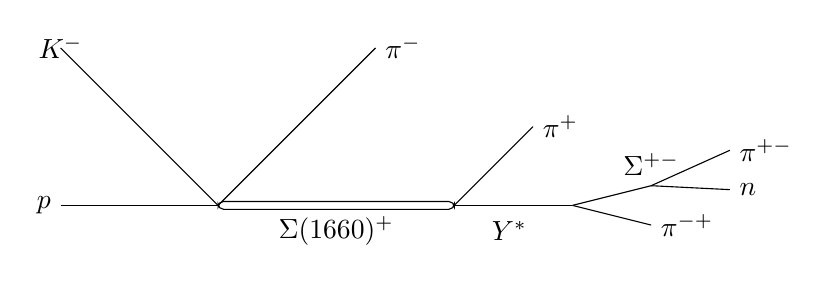
\begin{tikzpicture}
    \draw (-2.0, 2.0) node {$K^-$} -- (0, 0);
    \draw (-2.0, 0.0) node [left] {$p$} -- (0, 0);

    \draw (0, 0) -- (2.0, 2.0) node [right] {$\pi^-$};
    \draw (3.0, 0) -- (4.0, 1.0) node [right] {$\pi^+$};

    \draw [rounded corners=2pt] (0, 0.05) -- (3.0, 0.05) -- (3.0, -0.05) -- (0, -0.05) --cycle;
    \node (Sigma+) at (1.5, -0.33) {$\Sigma(1660)^+$};

    \draw (3.0, 0) -- (4.5, 0);
    \node (Y*) at (3.7, -0.33) {$Y^*$};

    \draw (4.5, 0) -- (5.5,  0.25) node [above] {$\Sigma^{+-}$};
    \draw (4.5, 0) -- (5.5, -0.25) node [right] {$\pi^{-+}$};

    \draw (5.5, 0.25) -- (6.5,  0.7) node [right] {$\pi^{+-}$};
    \draw (5.5, 0.25) -- (6.5,  0.2) node [right] {$n$};
  \end{tikzpicture}
  \caption{Decay chain of $K^- p \rightarrow \pi^- \Sigma^+(1660) \rightarrow \pi^- \pi^+ Y^* \rightarrow \pi^- \pi^+ (\pi \Sigma)^0$}
\end{figure}

The $\Lambda(1405)$ is a hyperon with strangeness $S=-1$, isospin $I=0$ and spin and spin parity $J^P=(\frac{1}{2})^-$.
In the Particle Data Group (PDG) \cite{PDG}, the mass and the width of the $\Lambda(1405)$ are assigned to $1405.1^{+1.3}_{-1.0}$MeV and $50.5\pm 2.0$MeV respectively,
based on several papers \cite{Dalitz, HADES_pheno, Esmaili}. 

The existence of the $\Lambda(1405)$ was predicted for the first time by R. H. Dalitz and S. F. Taun in 1959 as a quasi-bound state of $\bar{K}N$ \cite{Dalitz_1st}. 
The candidate was reported in the $K^- p\rightarrow \pi \pi \pi \Sigma$ reaction at the Lawrence Radiation Laboratory in 1961 \cite{L1405_LRL}.
The excess was reported in the neutral $\pi \Sigma$ spectrum, $K^- p \rightarrow \pi^{\pm} \pi^{\mp} (\pi \Sigma)^0$,
in the $\Lambda(1405)$ region compared to the doubly charged spectrum, $K^- p \rightarrow \pi^+ \pi^+ (\pi^- \Sigma^-$) or $K^- p \rightarrow \pi^- \pi^- (\pi^+ \Sigma^+$), in this paper.
However, there was not enough statistical data to discuss lineshape.

In order to solve these problems, R. J. Hemingway reported high-statistics $\pi^+ \Sigma^-$ and $\pi^- \Sigma^+$ spectra
using the $K^- p \rightarrow \pi^- \Sigma^+(1660) \rightarrow \pi^- \pi^+ (\pi^\mp \Sigma^\pm)$ with 4.2 GeV$/c$ $K^-$ beam \cite{Hemingway}.
In these spectra, the momentum transfer was restricted to, $t(K^-, \pi^-)<$1.0 GeV$/c$, in order to increase the purity of $\Sigma^+(1660)$.
As a result, the $\Sigma^+ \rightarrow \pi^0 p$ decay event of the $K^- p \rightarrow \pi^- \Sigma^+(1660) \rightarrow \pi^- \pi^+ (\pi^- \Sigma^+)$ reaction
gave a $\pi^- \Sigma^+$ spectrum with almost no background.
R. H. Dalitz and A. Deloff obtained the mass and width of the $\Lambda(1405)$ as $1406.4 \pm 4.0$ MeV and $50\pm 2$ MeV \cite{Dalitz}
by adapting the M-matrix method to this spectrum, and these parameters were adopted for the PDG.
On the other hand, the $\pi^+ \Sigma^-$ spectrum of the $K^- p \rightarrow \pi^- \Sigma^+(1660) \rightarrow \pi^- \pi^+ (\pi^+ \Sigma^-)$ reaction
had a background due to the ambiguity of the origin of the $\pi^-$.
Thus, the mass spectrum of $\Lambda(1405)$ was investigated using the $K^- p$ reaction with pion emission.

